\chapter{Internet as a Service}
\section{Virtualizzazione}
\textbf{IaaS} significa creare macchine virtualizzate per i nostri servizi.\
La virtualizzazione è un ``livello di astrazione'':\ il sistema operativo non deve più essere associato al server/PC su cui viene eseguito, viene quindi astratto dall'hardware, cioè non è installato direttamente sull'hardware.\
\begin{itemize}
    \item \textbf{Server virtualization}:\ livello di virtualizzazione tra il server fisico e il sistema operativo normalmente installato.
    \item \textbf{Macchine virtuali}:\ dove vengono effettivamente installati i sistemi operativi e le applicazioni.
\end{itemize}

\begin{figure}[H]
    \centering
    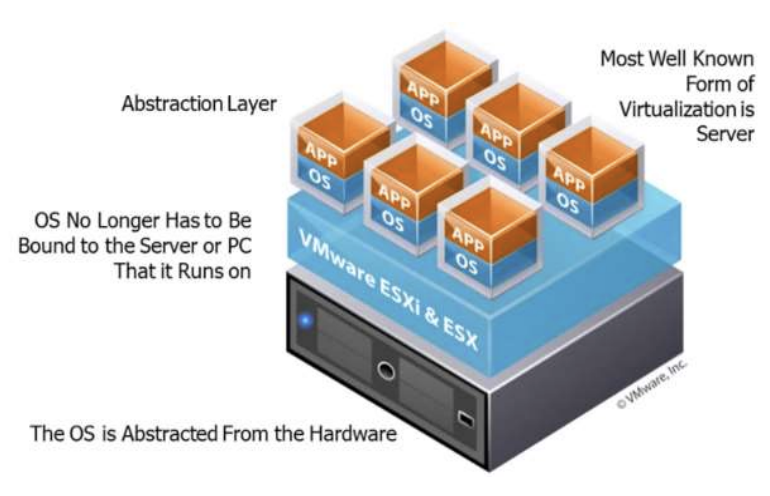
\includegraphics [width=0.5\textwidth]{immagini/model_virtualization.png}
    \caption*{Modello di virtualizzazione}
    \label{fig:model_virtualization}
\end{figure}

\noindent Un \textbf{Hypervisor} crea il livello di virtualizzazione e contiene il Virtual Machine Manager (VMM).\
Si possono distinguere due tipi di Hypervisor, il type 1 viene caricato direttamente sull'HW, il type 2 viene caricato su un sistema operativo in esecuzione sull'HW.\
Il type 2 ha un rapporto di consolidamento maggiore/minore rispetto al type 1.\
Type 1 per data center, type 2 per desktop/laptop.

\subsection{Amazon Elastic Compute Cloud (EC2)}

Amazon Elastic Cloud Computing mette a disposizione server virtuali (istanze) in modo semplice, veloce e economico.\
La scelta del tipo d'istanza e template da utilizzare (Windows/Linux) e il numero d'istanze avviene in modo semplice con AWS management console (o interfaccia grafica).\
Ci sono vari tipo di istanze a seconda delle proprie esegenze e diverse modalità di pagamento
\begin{itemize}
    \item \textbf{On demand}:\ ci sono molte opzioni che possiamo scegliere e ognuna ha un costo orario.
    \item \textbf{Reserved Instances}:\ significa di riservare delle instanze.
    \item \textbf{Spot Instances}:\ ci sono diversi tipo di offerte perché ci sono delle istanze che non vengono utilizzate nei datacenter.
    \item \textbf{Dedicated hosts}:\ esiste la possibilità anche di affittare un intero server per il nostro uso.
\end{itemize}
Tra le altre proprietà abbiamo lo storage persistente, Amazon Elastic Block Store (EBS), e l'autoscaling.

\begin{figure}[H]
    \centering
    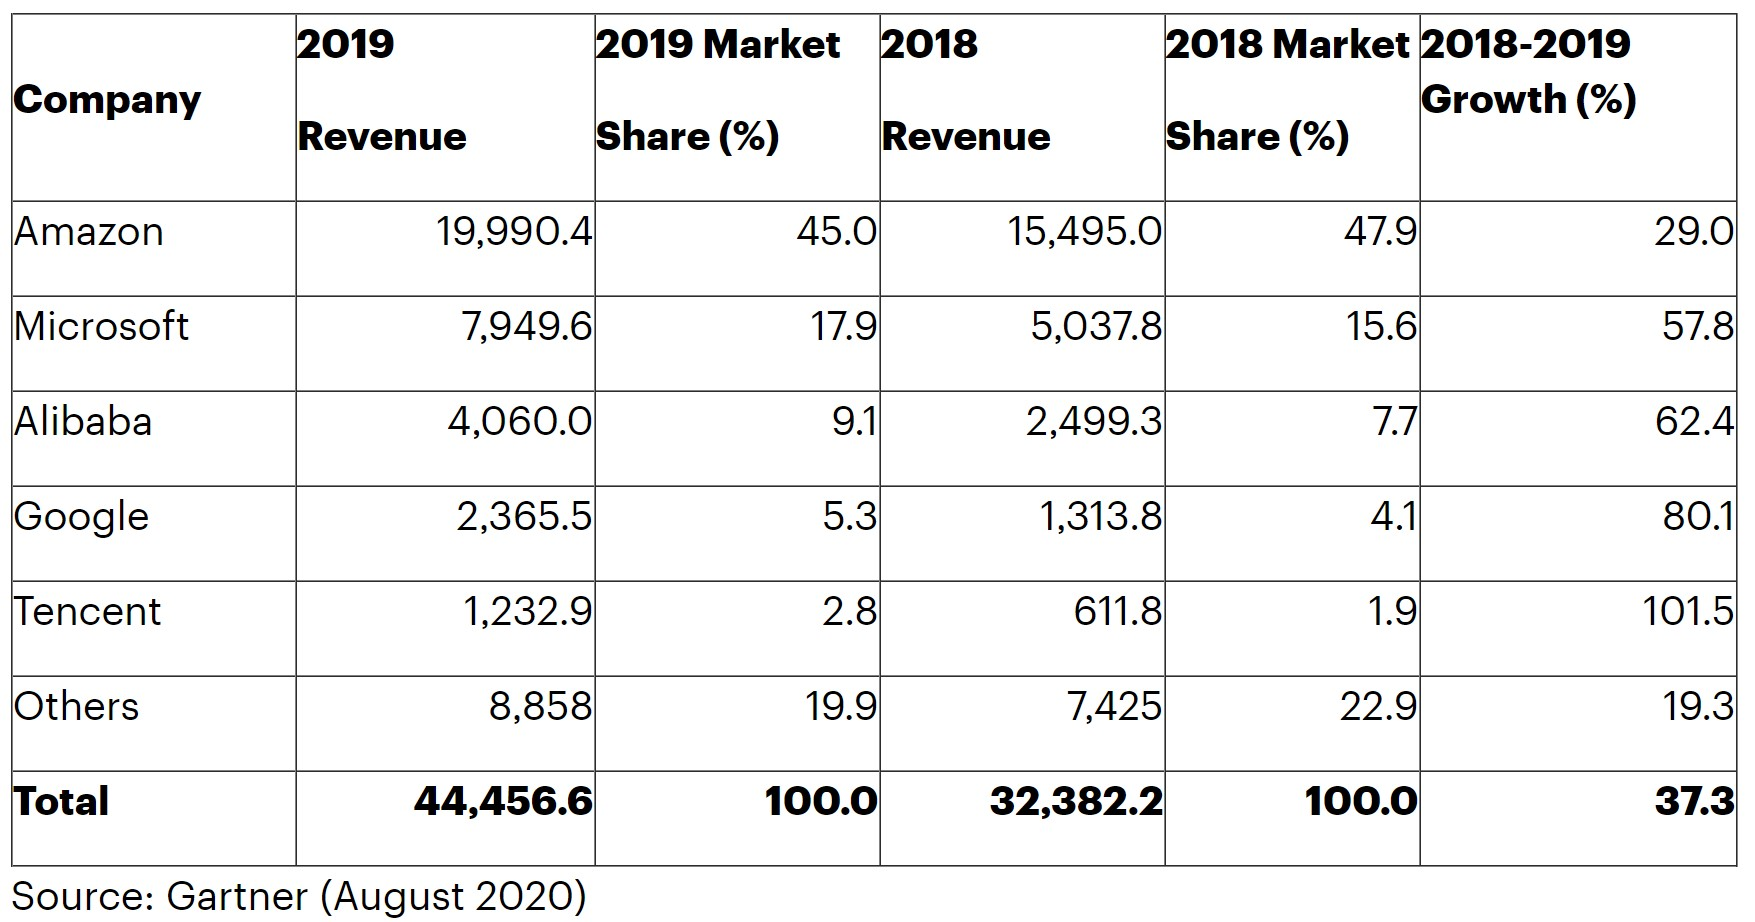
\includegraphics[width=\textwidth]{immagini/MarketShare.jpg}
    \caption*{IaaS Market share}
\end{figure}

\subsection{Amazon Simple Storage Service (S3)}
\begin{center}
    ``\textit{Everything must be made as simple as possible}.\
    \textit{But not simpler}.''
\end{center}
L'obiettivo di Amazon Simple Storage Service è quello di offrire un servizio virtualizzato per l'archiviazione dei dati più semplice possibile.\

Amazon presenta l'idea di avere dei ``\textit{bucket}'' (secchi) dove uno può trascinare i suoi dati.\
Mette a disposizione un'interfaccia grafica e permette di utilizzare il drag-and-drop per spostare i dati.\

Amazon S3 effettua backup dei dati per evitare la perdita e mantiene una copia delle versioni dei dati per permettere il loro recupero.\
Abbiamo diversi piani:
\begin{itemize}
    \item S3 Standard:\ si accede abbastanza frequentemente ai dati.
    \item S3 Infrequent Access:\ si accede poco frequentemente.
    \item Amazon Glacier:\ non si accede quasi mai, per esempio backup di database.
\end{itemize}
Per quanto riguarda la sicurezza offre una connessione SSL per la trasmissione dei dati e quindi per evitare che utenti malevoli catturino le nostre informazioni.

\subsection{Amazon Elastic Block Store}
Gli \textbf{Amazon Elastic Block Store} sono volumi di storage a blocchi persistenti da utilizzare con le istanze Amazon EC2 nel cloud AWS.\
Ogni volume Amazon EBS viene replicato automaticamente all'interno della sua zona di disponibilità per proteggerlo dal guasto dei componenti, offrendo alta disponibilità e durata.\

Progettato per carichi di lavoro delle applicazioni che traggono vantaggio dalla messa a punto di prestazioni, costi e capacità (ad esempio, analisi dei big data, elaborazione di flussi, data warehousing).\

\subsection{Dropbox}
È un servizio di file hosting che offre spazio di archiviazione gratuito, sincronizzazione dei file e strumenti di collaborazione (Dropbox Paper) a tutti.\
Inizialmente si trattava di un servizio che si interponeva tra Amazon e l'utente:\ Dropbox si occupava di prendere i file caricati dagli utenti e li inseriva in un bucket di S3.\

\subsubsection{L'esodo di Dropbox}

Dropbox è stato fondato nel 2007 da due studenti del MIT, avevano pensato di offrire gratuitamente spazio di archiviazione con limitazioni, e chi voleva poteva acquistare l'account premium per avere più capacità di memorizzazione.\
A Marzo 2016 Dropbox aveva 500 milioni di utenti.\

Per i primi otto anni della sua vita, Dropbox ha archiviato miliardi e miliardi di file su Amazons S3 (file su S3, metadati sulle proprie macchine).\

Tra il 2014 e il 2016, Dropbox ha costruito la propria vasta rete di computer e ha spostato il proprio servizio su una nuova generazione di macchine progettate dai propri ingegneri.\
La migrazione è stata una sfida molto grande dal punto di vista
\begin{itemize}
    \item \textbf{tecnico}:\ è stato progettato dell'hardware ad-hoc (``Diskotech'') per memorizzare quantità grande di dati con un nuovo codice chiamato ``Magic Pocket'';
    \item \textbf{logistico}:\ è stato necessario trasferire molti dati da Amazon S3 alla nuova infrastruttura.\ Inoltre andavano costruiti i datacenter;
    \item \textbf{contrattuale}:\ le deadline dei contratti dovevano essere rispettate per non rinnovare il contratto.
\end{itemize}
Vantaggi:
\begin{itemize}
    \item Autonomia (non dipendere da altro fornitore)
    \item Costi meno elevati per fornire il servizio (a regime)
    \item Possibilità offrire in modo più flessibile ed efficiente il servizio
    \item Supporto tecnico più veloce (in casa)
\end{itemize}
Svantaggi:
\begin{itemize}
    \item Costi elevati sia per realizzazione DC e migrazione
    \item Rischio elevato per competenze da acquisire
    \item Rischio elevato per perdita utenti durante migrazione o anche dopo
\end{itemize}
